\setboolean{IsHalfPage}{false}%
\setboolean{IsHalfPageLeftCol}{false}%
\setboolean{IsHalfPageRightCol}{false}%
\def\ChapterTitle{%
	Hawker Center Jakarta Experimental
}
\def\ChapterUrl{%
	https://arnottferels.github.io/work/hawker-center-jakarta-experimental
}
\def\ChapterDescription{%
	Innovative Concepts \& Designs Emerging from Thematic Experimentation
}
\def\ChapterDetailsLine{%
	Bachelor's Experimental Studio -- 2019 | Experimental Design; Parametric Design; Tensile Structures | West Jakarta, Indonesia
}
\def\ChapterDetailsTabular{%
	\begin{tabular}{@{}ll}
		\textbf{Type}        & Individual work                                                                  \\
		\textbf{Software}    & Rhino, Grasshopper, Kangaroo 2, Paneling Tools, Lumion, Photoshop \& Illustrator \\
		\textbf{Instructors} & Trianzani Sulshi \& Audrey Juliana                                               \\
		\textbf{URL}         & \textcolor{blue}{\footnotesize\texttt{\href{\ChapterUrl}{\ChapterUrl}}}          \\
	\end{tabular}
}
\def\ChapterAbstract{%
	This project relocates informal street vendors from West Jakarta along Letjen. S. Parman Rd, using experimental architectural exploration to create multi-dimensional spatial definition. Featuring a floating acrylic vista for zone and circulation definition, the design addresses challenges of limited green space and diverse zones near the busy road. Integrating experimental layers, materials, and facades, the Hawker Center creatively tackles the district's shortage of public spaces and green areas. The split structure incorporates elements like a steel frame, polycarbonate panels, and tensile structures, enhancing architectural creativity and the urban environment.
}
\StartTwoColumnLayout
\chapter*{\ChapterTitle}\addcontentsline{toc}{chapter}{\ChapterTitle}
\ChapterSetTocAddData{\ChapterDetailsLine}
\ChapterSetDetailsData{\ChapterDescription}{\ChapterDetailsLine}{\ChapterDetailsTabular}
\RuleAbstract
\ChapterAbstract
\section*{
  Site Analysis
 }
\vspace{0pt}
\setlength{\columnsep}{0.25cm}
\begin{multicols}{3}
	%
\begin{figure}[H]
	\centering
	\caption*{%
		Zoning
	}
	\includesvg[width=\linewidth]{src/graphics/hawker-center-jakarta-experimental--site-analysis-zoning.svg}
	\label{
		fig:hawker-center-jakarta-experimental--site-analysis-zoning
	}
\end{figure}

	%
\begin{figure}[H]
	\centering
	\caption*{%
		Circulation
	}
	\includesvg[width=\linewidth]{src/graphics/hawker-center-jakarta-experimental--site-analysis-circulation.svg}
	\label{
		fig:hawker-center-jakarta-experimental--site-analysis-circulation
	}
\end{figure}

	%
\begin{figure}[H]
	\centering
	\caption*{%
		Greenary
	}
	\includesvg[width=\linewidth]{src/graphics/hawker-center-jakarta-experimental--site-analysis-greenery.svg}
	\label{
		fig:hawker-center-jakarta-experimental--site-analysis-greenery
	}
\end{figure}

\end{multicols}
The site is positioned adjacent to the vibrant Letjen S. Parman road, extending from the West to the South. It is surrounded by diverse zones, including commercial, government, and residential areas. The vicinity comprises various road types, ranging from expansive highways to smaller local ones, emphasizing the significance of mobility considerations. Tall buildings with mixed functions encompass most sides, while shorter residential structures are situated on the Northern and Eastern sides. Unfortunately, there is limited green space in the area.
\vfill
%
\begin{figure}[H]
	\centering
	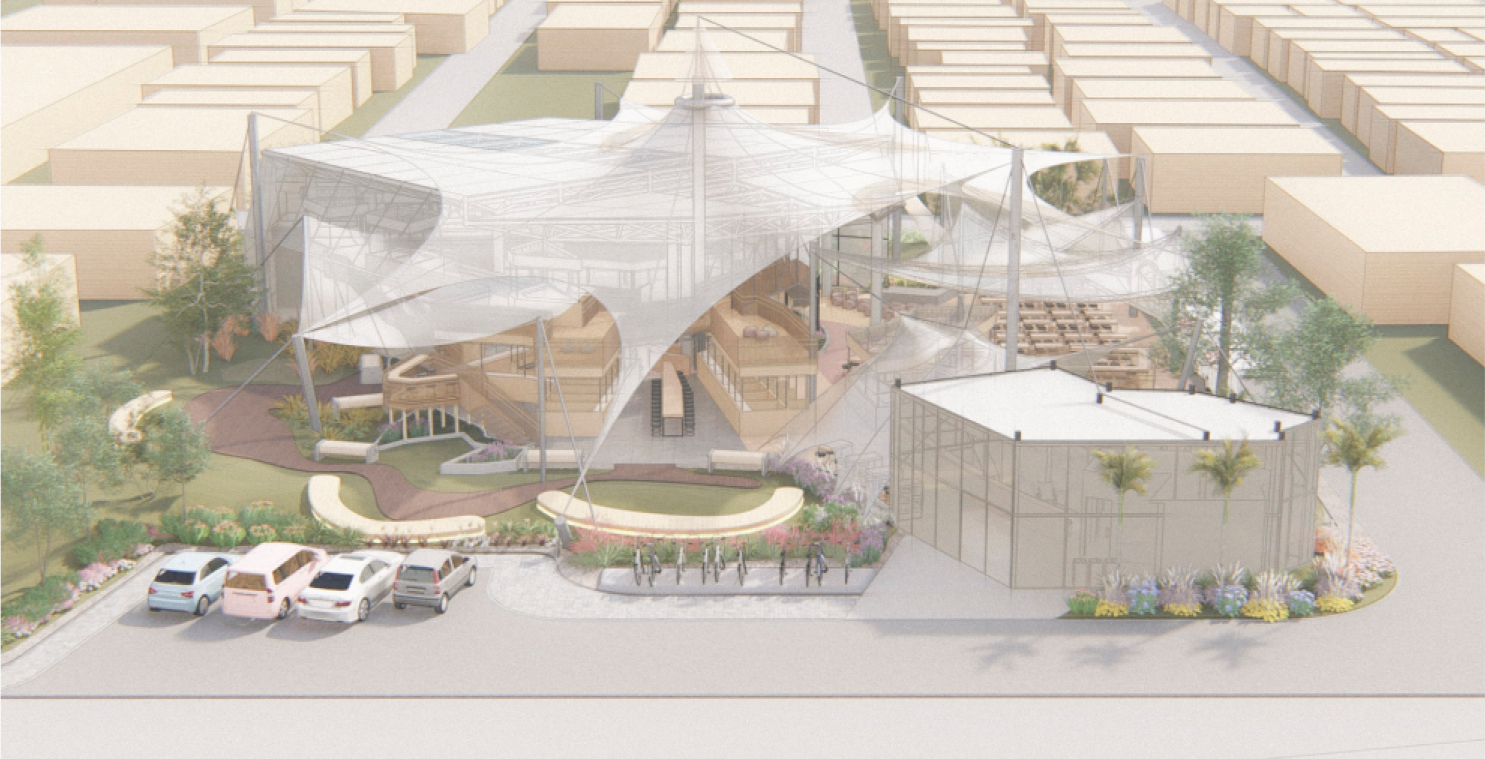
\includegraphics[width=\linewidth]{src/graphics/hawker-center-jakarta-experimental--perspective-aerial-view.jpg}
	\caption*{%
		Aerial view -- Hawker Center Jakarta Experimental
	}
	\label{
		fig:hawker-center-jakarta-experimental--perspective-aerial-view
	}
\end{figure}

\columnbreak%
\begin{minipage}[t][\textheight][t]{\linewidth}
	\section*{
	  Experimental Architectural Exploration -- From Abstraction to Form
	 }
	\begin{center}
		\begin{minipage}[t]{0.8125\linewidth}
			\newcommand{\FigureHawkerCenterJakartaExperimentalStep}[4]{%
				\begin{figure}[H]
					\centering
					\captionof*{figure}{%
						\footnotesize
						\textcolor{black}{%
							\textnormal{%
								\textbf{#2}
								\hspace{0.25cm}
								\parbox{0.8\linewidth}{%
									\textbf{#3}\\%
									\noindent#4%
								}
							}
						}
					}
					\vspace{0.125cm}
					#1%
					\label{fig:hawker-center-jakarta-experimental--step-#2}
				\end{figure}
			}
			\def\Figure{\FigureHawkerCenterJakartaExperimentalStep}
			\setlength{\MinipageGap}{0.5cm}
			\setlength{\MinipageAWidth}{\dimexpr0.45\linewidth -\MinipageGap}
			\setlength{\MinipageBWidth}{\dimexpr\linewidth -\MinipageAWidth -\MinipageGap\relax}
			\begin{minipage}[t]{\MinipageAWidth}%
				\Figure{%
					\includesvg[width=\linewidth]{src/graphics/hawker-center-jakarta-experimental--step-1.svg}
				}%
				{1}%
				{Daydream Spaces}%
				{Creating abstract geometry with annotated printouts crafted from cut verbs and nouns.}%
			\end{minipage}%
			\hspace{\MinipageGap}%
			\begin{minipage}[t]{\MinipageBWidth}%
				\Figure{%
					\includesvg[width=\linewidth]{src/graphics/hawker-center-jakarta-experimental--step-2.svg}
				}%
				{2}%
				{Dance and Space}%
				{Forming dance movement with clay.}%
			\end{minipage}%
			\vfill
			\begin{minipage}[t]{\MinipageAWidth}%
				\Figure{%
					\includesvg[width=\linewidth]{src/graphics/hawker-center-jakarta-experimental--step-3.svg}
				}%
				{3}%
				{Open Text}%
				{Crafting acrylic plans to shape spatial divisions.}%
			\end{minipage}%
			\hspace{\MinipageGap}%
			\begin{minipage}[t]{\MinipageBWidth}%
				\Figure{%
					\includesvg[width=\linewidth]{src/graphics/hawker-center-jakarta-experimental--step-4.svg}
				}%
				{4}%
				{Space Aggregation}%
				{Creating an intriguing aggregation derived from Steps 1, 2 \& 3.}%
			\end{minipage}%
			\vfill
			\setlength{\MinipageAWidth}{\dimexpr0.3\linewidth -\MinipageGap}
			\setlength{\MinipageBWidth}{\dimexpr0.4\linewidth -\MinipageGap}
			\setlength{\MinipageCWidth}{\dimexpr\linewidth -\MinipageAWidth -\MinipageBWidth -\MinipageGap\relax}
			\begin{minipage}[t]{\MinipageAWidth}%
				\Figure{%
					\includesvg[width=\linewidth]{src/graphics/hawker-center-jakarta-experimental--step-5.svg}
				}%
				{5}%
				{Architectural Notation}%
				{Symbolically representing architectural concepts in 2D.}%
			\end{minipage}%
			\hspace{\MinipageGap}%
			\begin{minipage}[t]{\MinipageBWidth}%
				\Figure{%
					\includesvg[width=\linewidth]{src/graphics/hawker-center-jakarta-experimental--step-6.svg}
				}%
				{6}%
				{Multi-dimensional}%
				{Defining spatial zones unexpectedly in 3D from the 2D of step 5.}%
			\end{minipage}%
			\hspace{\MinipageGap}%
			\begin{minipage}[t]{\MinipageCWidth}%
				\Figure{%
					\includesvg[width=\linewidth]{src/graphics/hawker-center-jakarta-experimental--step-7.svg}
				}%
				{7}%
				{Movement as Circulation}%
				{%
					Defining spatial flow and circulation from its main axes.
				}%
			\end{minipage}%
			\vfill
			\setlength{\MinipageAWidth}{\dimexpr0.45\linewidth -\MinipageGap}
			\setlength{\MinipageBWidth}{\dimexpr\linewidth -\MinipageAWidth -\MinipageGap\relax}
			\begin{minipage}[t]{\MinipageAWidth}%
				\Figure{%
					\includesvg[width=\linewidth]{src/graphics/hawker-center-jakarta-experimental--step-8.svg}
				}%
				{8}%
				{Layer and Function}%
				{Determining experimental layers and integrating functions.}%
			\end{minipage}%
			\hspace{\MinipageGap}%
			\begin{minipage}[t]{\MinipageBWidth}%
				\Figure{%
					\includesvg[width=\linewidth]{src/graphics/hawker-center-jakarta-experimental--step-9.svg}
				}%
				{9}%
				{Structures and Materials}%
				{Defining architectural elements and material palette based on representative materials.}%
			\end{minipage}%
			\vfill
			\begin{minipage}[t]{\MinipageAWidth}%
				\Figure{%
					\includesvg[width=\linewidth]{src/graphics/hawker-center-jakarta-experimental--step-10.svg}
				}%
				{10}%
				{Façade Framework}%
				{Determining the form and geometric face patterns.}%
			\end{minipage}%
			\hspace{\MinipageGap}%
			\begin{minipage}[t]{\MinipageBWidth}%
				\Figure{%
					\includesvg[width=\linewidth]{src/graphics/hawker-center-jakarta-experimental--step-11.svg}
				}%
				{11}%
				{Photogrammetric Analysis}%
				{Architectural evaluation through photogrammetry \& documentation.}%
			\end{minipage}%
		\end{minipage}
	\end{center}
	\vfill
	This architectural workshop delves into themes such as abstract geometry, dance movement, spatial aggregation, and architectural notation through experimental exercises. We engage in manipulating materials, creating layers, and evaluating structures using photogrammetry to foster creativity and innovation in architectural design.
\end{minipage}
\newpage
\section*{
  Design Strategy
 }
\begin{center}
	\vspace{-\baselineskip}%
	\begin{minipage}[t]{0.8\linewidth}
		%
\begin{figure}[H]
	\centering
	\includesvg[width=\linewidth]{src/graphics/hawker-center-jakarta-experimental--design-strat.svg}
	\label{
		fig:hawker-center-jakarta-experimental--design-strat
	}
\end{figure}

	\end{minipage}
\end{center}
\vspace{-\baselineskip}%
\vfill
\section*{
  Programs
 }
%
\begin{figure}[H]
	\centering
	\includesvg[width=\linewidth]{src/graphics/hawker-center-jakarta-experimental--plans.svg}
	\label{
		fig:hawker-center-jakarta-experimental--plans
	}
\end{figure}

\vfill
The initial level includes public F\&B stalls, food courts, and dining areas. The Northeast section hosts a private service area. Additionally, mini F\&B stalls and conference rooms on the first floor create a semi-private character.
\vfill
%
\begin{figure}[H]
	\centering
	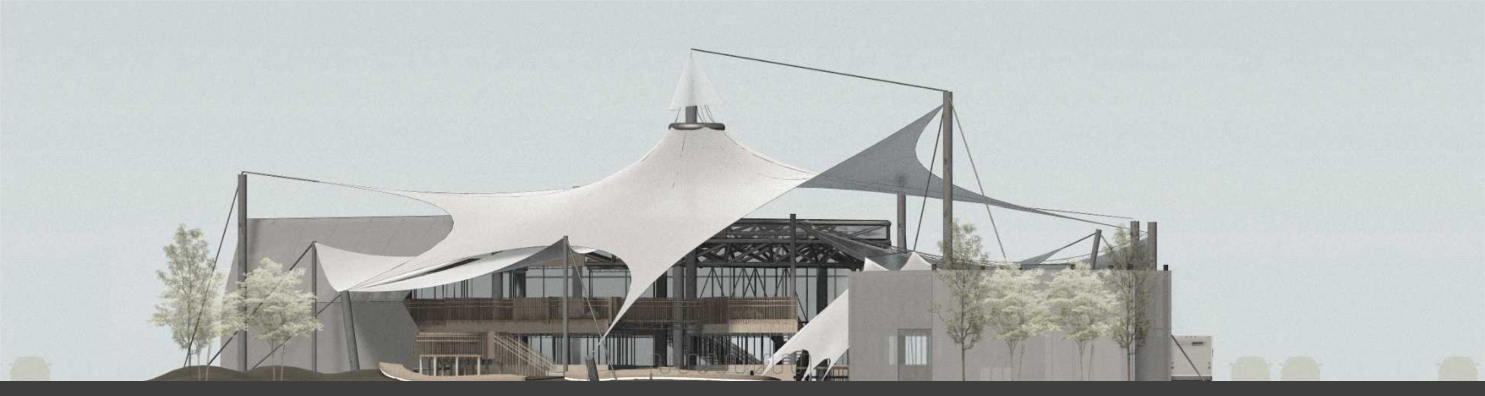
\includegraphics[width=\linewidth]{src/graphics/hawker-center-jakarta-experimental--perspective-front-elevation-southwest.jpg}
	\caption*{%
		Front elevation (Southwest)
	}
	\label{
		fig:hawker-center-jakarta-experimental--perspective-front-elevation-southwest
	}
\end{figure}

\columnbreak%
\section*{
  Programs \textit{(cont.)}
 }
\begin{center}
	\vspace{-\baselineskip}%
	\begin{minipage}[t]{0.825\linewidth}
		%
\begin{figure}[H]
	\centering
	\includesvg[width=\linewidth]{src/graphics/hawker-center-jakarta-experimental--programs-axonometric.svg}
	\label{
		fig:hawker-center-jakarta-experimental--programs-axonometric
	}
\end{figure}

		\vfill
		The structure is split into two primary segments: the front, designated for public use, and the rear, allocated for private and service purposes. A commercial zone and public space are positioned between these two segments.
	\end{minipage}
\end{center}
\vfill
\setlength{\columnsep}{0.25cm}
\begin{multicols}{2}
	%
\begin{figure}[H]
	\centering
	\includesvg[width=\linewidth]{src/graphics/hawker-center-jakarta-experimental--perspective-bicycle-park.svg}
	\caption*{%
		Bicycle park
	}
	\label{
		fig:hawker-center-jakarta-experimental--perspective-bicycle-park
	}
\end{figure}

	%
\begin{figure}[H]
	\centering
	\includesvg[width=\linewidth]{src/graphics/hawker-center-jakarta-experimental--perspective-food-court.svg}
	\caption*{%
		Food court
	}
	\label{
		fig:hawker-center-jakarta-experimental--perspective-food-court
	}
\end{figure}

	%
\begin{figure}[H]
	\centering
	\includesvg[width=\linewidth]{src/graphics/hawker-center-jakarta-experimental--perspective-food-court-atrium.svg}
	\caption*{%
		Food court (atrium)
	}
	\label{
		fig:hawker-center-jakarta-experimental--perspective-food-court-atrium
	}
\end{figure}

	%
\begin{figure}[H]
	\centering
	\includesvg[width=\linewidth]{src/graphics/hawker-center-jakarta-experimental--perspective-main-entrance.svg}
	\caption*{%
		Main entrance
	}
	\label{
		fig:hawker-center-jakarta-experimental--perspective-main-entrance
	}
\end{figure}

\end{multicols}
\EndTwoColumnLayout
\newpage
